% coding:utf-8

% Ausführen in R: 
% Sweave("C:/Daten/Daniel/studium/git_repo/sem2/stoc/sw07/sw07_5.Rnw",encoding='UTF-8')

\section{Aufgabe 4}

\subsection{a}
\begin{Schunk}
\begin{Sinput}
> iron.all<-read.table("ironF3.dat",header=TRUE)
> iron<-iron.all[,-1]
> boxplot(iron)
\end{Sinput}
\end{Schunk}
\includegraphics{sw07_5-001}

\subsection{b}
\begin{Schunk}
\begin{Sinput}
> iron.log=log10(iron)
> boxplot(iron.log)
\end{Sinput}
\end{Schunk}
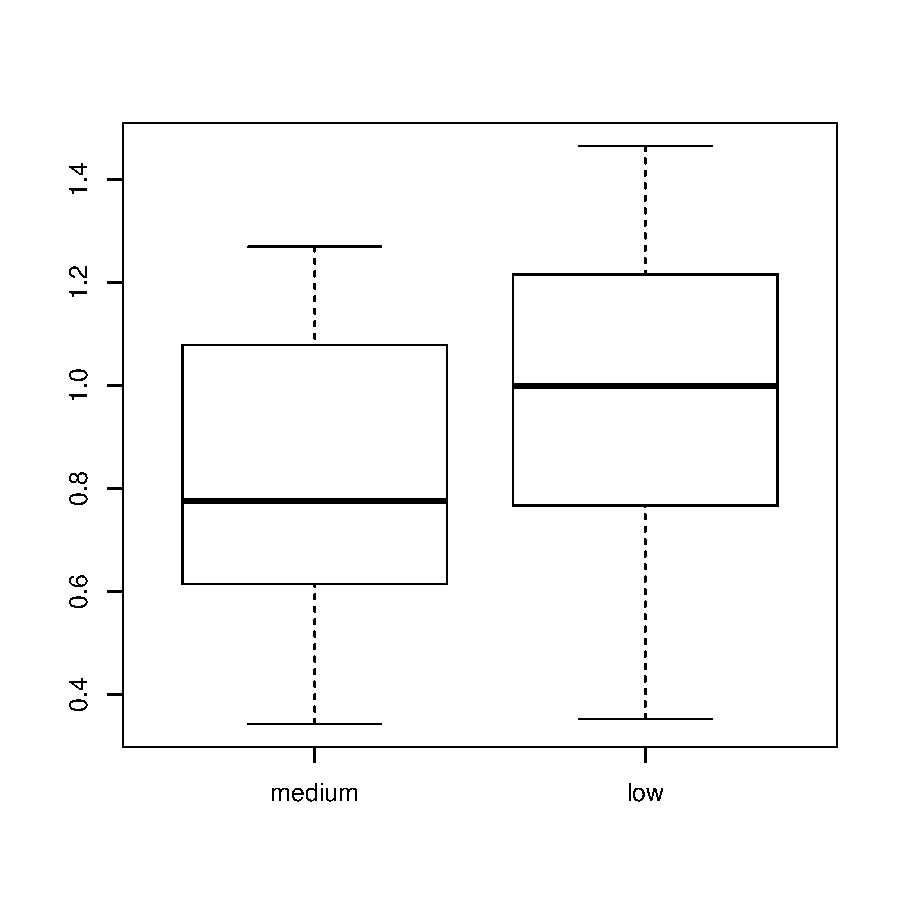
\includegraphics{sw07_5-002}

\subsection{c}
\begin{Schunk}
\begin{Sinput}
> iron.med<-iron[1]
> iron.log.med<-iron.log[1]
> plot(1:nrow(iron.med),iron.med)